\levelB{Experiment on random data detection}
\label{sec:exprandom}

In the previous sections, it was observed that the higher the number of classes being considered during the creation of a file fragment classification model, the higher is the error rate of this model. In addition, the comparison of pairs of classes indicated that high entropy data structures may be responsible by some part of those errors.

Prior to conducting experiments to find the major cause of error, a list of conceivable error sources (E1 to E4) was elaborated:
\begin{enumerate}[itemindent=\parindent,label=\textbf{E\arabic*.}]
    \item For some data structure, the model cannot distinguish it from random data. This can happen if the pattern in the data is too complex, beyond the capabilities of the model. It may be the case that in practice no model can perform this distinction or, instead, this may be a limitation of this particular model only. This situation may occur in files that use compression or cryptography, or more generally, any file type with high entropy.

    \item Different file types using the same data structure. It is common to a given file type to employ different types of data structures. If two or more file types make use of the same data structure, the existence of that structure will then not be sufficient to differentiate those file types, as it may belong to anyone of them.
    The reverse, a file type that uses multiple kinds of data structures, does not constitute a problem as it simply results in extra work during the model training.

    \item Same file type with multiple extensions. If the same file type appears in the dataset with multiple extensions, ``JPG'' and ``JPEG'' for example, the model will not be able to predict which label is used in the validation dataset for a given instance, since this distinction exists in the labelling but not in the content.

    \item Files that contain other files. Some file types need to embed other files. If the inner file is categorized, even if the model finds an unmistakable pattern, it will not match the label, which will be the extension of the outer file. A ``PDF'' file, for example, can embed a ``JPG'' file. If the model predict ``JPG'' as the class of a portion of this file, it will no match the instance label on the dataset, which would be ``PDF''.
\end{enumerate}

The first error source, E1, is the focus of this section. In the file fragment classification task, it is expected that some portion of the classifications errors of a given model be caused by its inability to recognize patterns in the data, if the data has high entropy. In these situations, even humans may be unable to tell if a sample is valid or if it is random data.

The three last error sources listed above, E2 to E4, are not explored in this study. They are similar in nature, as the last two may be viewed as special cases of E2. This error source comes from the practice of using the extension of the file as the class to each of its parts. An analogy with speech recognition would be to label each syllable of a spoken word using the word as its label and then try to predict the whole word using only a syllable.

Unfortunately, for the file fragmentation task the potential labels for smaller parts may be less obvious than it is for speech recognition. The best case scenario would be if the neural network itself could choose the labelling. But evaluating those predicted labels using labels of its own choosing would introduce bias, as it could prefer to create only easy labels. Saying that all file types are composed of ``data'' is correct, but it is unhelpful.

\levelC{Hypothesis}
The goal of this experiment is to test the hypothesis that part of the errors of file fragment classification  can be explained by the existence of data that has no structure detectable by the model. Not all file types possess this kind of data, and on those that do, they should compose only a portion of the file.


\levelC{Models}
For each file type, a new model is trained to classify a fragment into two classes, random or not random. The stopping condition used is 4 epochs without improvement in validation accuracy.
The same sampling, input, and output details described in section \ref{sec:evalmodels} were used here. The model that gave best results in that section, identified as ``CLD'', was selected to be used.


\levelC{Dataset}
The model training was divided in two passes, depicted in figure \ref{fig:randommeasure}. Each pass trains a different model for each filetype. In the first pass, the dataset creation for a given file type follows almost the same procedure mentioned in the previous section, but instead of selecting two file types, it selects one file type and uses a random data generator for the other class.

\noindent
\begin{figure*}[htb!]
\centering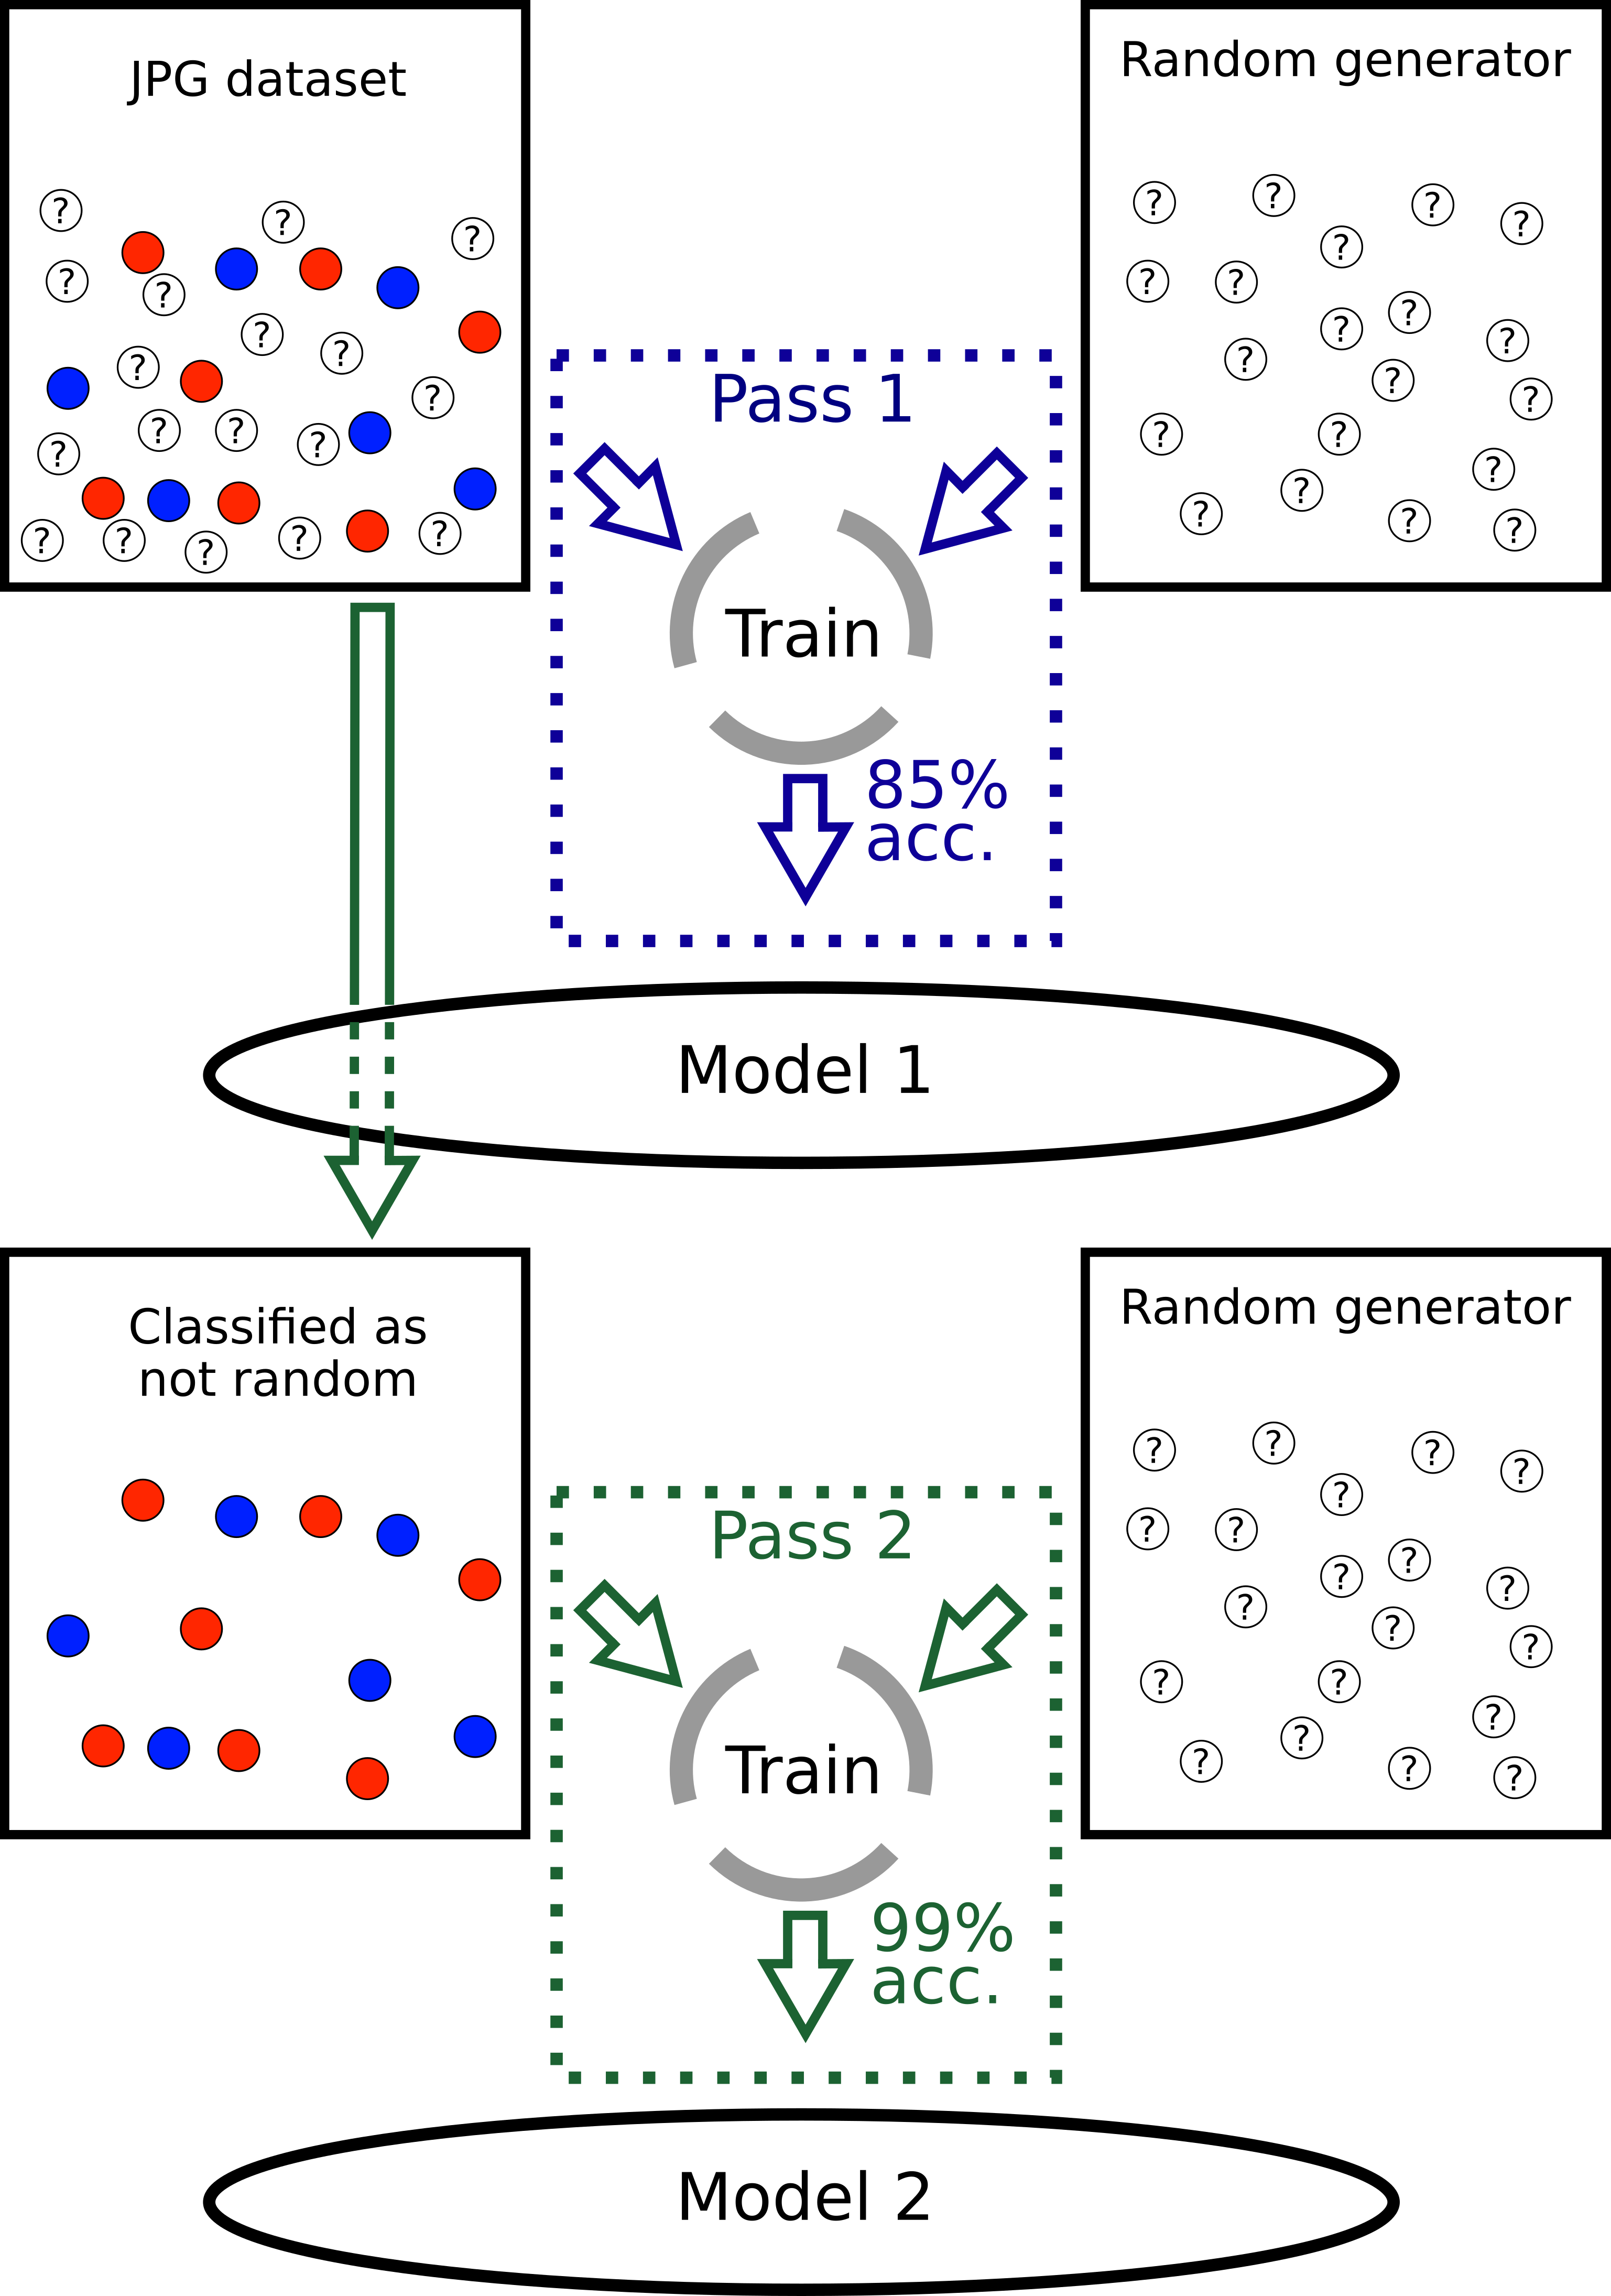
\includegraphics[width=0.50\textwidth]{content/random_measure.png}
\caption{\label{fig:randommeasure}Example of the random measure for the JPG file type. In pass 1, a model is trained to classify the data as ``random'' or ``not random'', achieving 87\% accuracy. In pass 2, another model is trained to do the same task, but the JPG blocks used are those classified as ``not random'' by model 1. As model 2 achieves an accuracy of 99\%, it validates that almost all the blocks classified as ``not random'' by model 1 are indeed not random. Then model 1 can be used to make an upper boundary estimate of the randomness of the dataset.}%
\end{figure*}

When the model training finishes, if the validation accuracy is above 98\% for a given file type, no further passes are required by that file type, as the model already can distinguish between ``random'' and ``not random'' classes for that particular file type. This will only happen on file types that have almost no random like structures.

In the second pass, the file type dataset is filtered and only those fragments classified as ``not random'' in the first pass are used in the second pass. The random generator needs no filtering. If in the second pass the accuracy is above 98\%, it means that the pass 1 was successfully selected samples that have almost no random like structures. In that case, the pass 1 model can then used in the original dataset, giving a count of how many fragments are correctly identified as not random.

\levelC{Results}
For some file types, training achieved an accuracy higher than 98\% on the first pass. These are the file types where a model should have no difficulty finding patterns. For the remaining file types, all achieved an accuracy higher than 98\% on the second pass, which is fortunate, as this avoids the need to use further passes and  simplifies calculations.

Figure \ref{fig:not_random} shows, for each file type, the percent of 512 byte fragments identified as not random, from a sample of 1000 fragments for each file type.

\noindent
\begin{figure*}[htb!]
\centering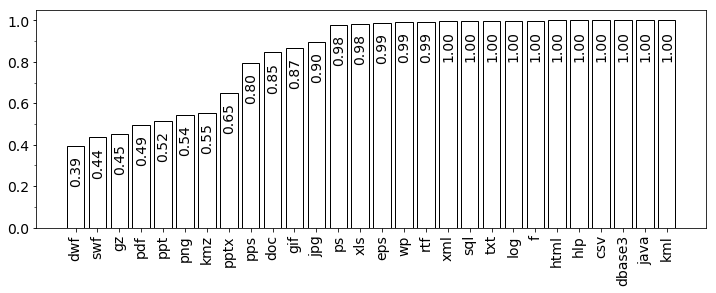
\includegraphics[width=0.50\textwidth]{content/random.png}
\caption{\label{fig:not_random}Validation accuracy of models trained to distinguish each file type from random data. The 90\% accuracy of JPG, for example, means that recognizable patterns were found on 90\% of the blocks of the JPG dataset.}%
\end{figure*}



\levelC{Limitations and threats to validity}
The procedure applied in this experiment avoids false positives over false negatives. In other words, it avoids random data classified as not random at the cost of missing potentially recognizable structures in valid fragments. Thus, it is expected that the exact valid fragments count, which is unknown in practice, will be higher than the number obtained. Taking the JPG file type as example, in which 90\% of the blocks were identified as ``not random'', this means that the true randomness value is some unknown value between 0 and 10\%.

\levelC{Discussion of results}

Having a minimum amount of recognizable structures for each file type, it is now possible to calculate the maximum amount of the classification errors that can be attributed to error cause E1, which happens when the complexity of the data is beyond the the model's capability to recognize patterns.

The mean accuracy for all file types, using data listed in figure \ref{fig:not_random}, is 83.5\%. Assuming a dataset with balanced classes, if all the blocks considered random data were misclassified, then the maximum amount of error due to data complexity would be 16.5\%. If all blocks considered random were classified as DWG, which is the class with less recognizable patterns, then the maximum amount of error would be 14.3\%.

% The extensions ``text'' and ``unk'' were also discarded because they do not correspond to a file type, and the files that use them belong to assorted types. 